% Static-circuit (Aurora) vs zkVM substrate — the decision-rule figure.
% Numbers: Aurora setup+prove 3.78 min (tab:aurora-ref, this thesis, Loquat-BDEC,
% lambda=80); zkVM PLUM-verify 14.25 min with precompile (Cell 2). Update churn:
% static N_circ,N_param >= 1 per phi-change; zkVM = 0 (Table churn).
% Compile: pdflatex substrate_compare.tex
\documentclass[border=4pt]{standalone}
\usepackage{tikz}
\usepackage{newtxtext,newtxmath}
\usetikzlibrary{positioning,arrows.meta,fit,backgrounds,calc}
\begin{document}
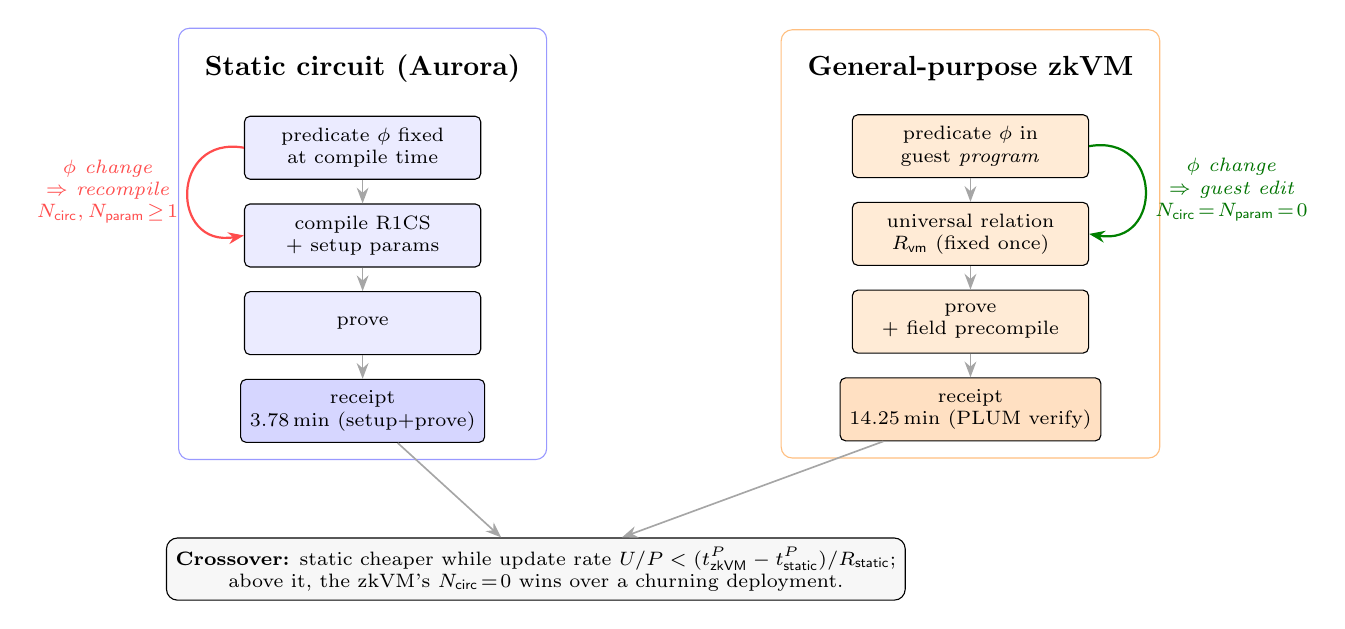
\begin{tikzpicture}[
  font=\small,>={Stealth[length=2mm]},
  hdr/.style={font=\bfseries},
  st/.style={draw,rounded corners=2pt,fill=blue!8,minimum width=30mm,minimum height=8mm,align=center,font=\scriptsize},
  vm/.style={draw,rounded corners=2pt,fill=orange!16,minimum width=30mm,minimum height=8mm,align=center,font=\scriptsize},
  note/.style={font=\scriptsize\itshape,gray},
  flow/.style={->,semithick,gray!70},
  chg/.style={->,thick,red!70},
]

% ===== left column: static circuit =====
\node[hdr] (sh) {Static circuit (Aurora)};
\node[st,below=3mm of sh] (sa) {predicate $\phi$ fixed\\at compile time};
\node[st,below=3mm of sa] (sb) {compile R1CS\\$+$ setup params};
\node[st,below=3mm of sb] (sc) {prove};
\node[st,below=3mm of sc,fill=blue!16] (sd) {receipt\\\scriptsize $3.78$\,min (setup+prove)};
\draw[flow] (sa)--(sb); \draw[flow](sb)--(sc); \draw[flow](sc)--(sd);
% phi change -> recompile loop
\draw[chg] (sa.west) to[out=170,in=190,looseness=2.2]
   node[left,note,align=center,red!70]{$\phi$ change\\$\Rightarrow$ recompile\\$N_{\mathsf{circ}},N_{\mathsf{param}}\!\ge\!1$} (sb.west);

% ===== right column: zkVM =====
\node[hdr,right=34mm of sh] (vh) {General-purpose zkVM};
\node[vm,below=3mm of vh] (va) {predicate $\phi$ in\\guest \emph{program}};
\node[vm,below=3mm of va] (vb) {universal relation\\$R_{\mathsf{vm}}$ (fixed once)};
\node[vm,below=3mm of vb] (vc) {prove\\\scriptsize $+$ field precompile};
\node[vm,below=3mm of vc,fill=orange!24] (vd) {receipt\\\scriptsize $14.25$\,min (PLUM verify)};
\draw[flow] (va)--(vb); \draw[flow](vb)--(vc); \draw[flow](vc)--(vd);
% phi change -> guest edit, no recompile
\draw[chg,green!50!black] (va.east) to[out=10,in=-10,looseness=2.2]
   node[right,note,align=center,green!45!black]{$\phi$ change\\$\Rightarrow$ guest edit\\$N_{\mathsf{circ}}\!=\!N_{\mathsf{param}}\!=\!0$} (va.east|-vb);

% ===== bottom: the decision rule =====
\node[draw,rounded corners,fill=gray!6,below=12mm of sd,xshift=22mm,
      minimum width=78mm,align=center,font=\scriptsize] (rule)
  {\textbf{Crossover:} static cheaper while update rate
   $U/P < (t^P_{\mathsf{zkVM}}-t^P_{\mathsf{static}})/R_{\mathsf{static}}$;\\
   above it, the zkVM's $N_{\mathsf{circ}}\!=\!0$ wins over a churning deployment.};
\draw[flow] (sd) -- (rule); \draw[flow] (vd) -- (rule);

\begin{scope}[on background layer]
  \node[fit=(sh)(sd),draw=blue!40,rounded corners,inner sep=6pt]{};
  \node[fit=(vh)(vd),draw=orange!50,rounded corners,inner sep=6pt]{};
\end{scope}
\end{tikzpicture}
\end{document}
